
\chapter{Introduction}

\label{ch:introduction}

\section{Motivation}

Reconfigurable system is a computing system which combines the flexibility of software with the high performance of hardware by deploying \gls{fpga} technology.
The structure of a reconfigurable system can be changed by the end-user after the manufacturing process or even at run-time.
The development of reconfigurable system has been driven largely by \glspl{fpga}, which are semiconductor devices with prefabricated logic and routing resources.
The functionality and interconnection of an \gls{fpga} can be reconfigured with any new design multiple times.
The reconfiguration enables application-specific tuning of designs and their adaptation to new standards.
This reconfigurability make \glspl{fpga} suited to prototyping \gls{asic} designs.
In recent years, there has been a significant increase in the size of \glspl{fpga}.
Modern state-of-the-art \glspl{fpga} contain numerous programmable logic cells, \glspl{dsp}, memory blocks, high-throughput transceivers, peripheral devices, customisable IP blocks and even micro-processor cores~\cite{alterasoc,xilinxzynq}.
These components enable higher integration level, faster execution speed and lower power consumption through tailor-made data-paths, increased fine-grained parallelism and better memory utilisation.
In addition, \gls{fpga} technology allows arbitrary precision floating-point arithmetic.
This allows for reduction of the circuit area or increases parallelism without significant impact to the accuracy of the results~\cite{chow11,chow12}.
~\gls{fpga} devices also support dynamic run-time reconfiguration enabling applications demanding adaptive and flexible hardware. 

The advantages mentioned above facilitate the use of ~\glspl{fpga} in \gls{hpc} and real-time computing.
\gls{hpc} has stringent speed, space and power consumption requirements.
Examples include weather forecasting, brain simulation and molecular dynamics simulation. 
In the last decade, researchers have extended the scope of \glspl{fpga} from prototyping to accelerating a wide variety of software, such as Monte Carlo simulation~\cite{chow12} and video processing~\cite{guo04}.
\glspl{fpga} show a lot of promise for \gls{hpc}.
Execution time and power consumption of applications running on \glspl{fpga} can be improved by up to several orders of magnitude compared to state-of-the-art microprocessors~\cite{chow11,chow12,craven07,guo04,pell11}.

%While the main requirement of ~\gls{hpc} is performance,
Real-time computing is driven by system being able to respond to input stimulus in finite intervals.
%focuses on meeting deadline which are finite and specified time intervals within which the system must respond to an input stimulus.
Failing a deadline can cause degraded quality of service and even a total system failure.
Real-time systems are found in a wide range of applications areas, from simple domestic appliances to financial systems, large scale process control and safety critical avionics.
Examples include air traffic management~\cite{crisostomi07,eele11}, unmanned aerial vehicles~\cite{ortiz06}, robotics~\cite{dellaert99}, and medical surgery~\cite{kwok10}.
In some applications, the required response times are measured in milliseconds, in others it is seconds or even minutes. 
Nevertheless, they all must be satisfied.

\glspl{fpga} are considered as a platform for embedded real-time applications where software tasks running on micro-processors coexist with hardware tasks running on reconfigurable logics~\cite{paul12,schoeberl08,whitham09,alteradoc}.
However, these implementations are software-based which means that multiple real-time tasks are managed by dedicated \gls{rtos} for reconfigurable devices.
Real-time tasks running on micro-processors have to consider problems resulting from complex architectures.
Pipelines, caches, branch prediction, or out-of-order execution result in complex state machines which to be managed by either software or hardware.
Extensive research has been conducted on micro-processor-based real-time applications regarding time predictability, \gls{wcet}, task scheduling and management~\cite{burns01,davis11,puschner00}.
%While the objective of real-time computing is to meet the timing requirement of each task rather than being fast, many real-time applications that involve \glspl{fpga} are implemented on embedded systems.
%Most of these systems utilise a single FPGA board together with a soft processor core, which provides limited performance for non-computed intensive applications.
%Even hardware logic components on \glspl{fpga} are occasionally used to offload the micro-processor, these implementations provide limited performance for non-compute intensive applications.
Nowadays, there are many real-time applications which push processing systems to their limit with the required response time.
Real-time needs can be extremely hard when a large amount of data have to be processed in a short period of time.
For example, high-frequency trading is becoming popular with execution time bounded to microseconds~\cite{mcgowan10}. 

\glspl{fpga} have potential to play an important role in high-performance real-time applications as they provide predictable timing performance, the ability to 
perform highly parallel calculations, better solution quality~\cite{chau13fpt,chau14fccm} and lower power consumption~\cite{chau13arc}.
For instance, in Monte Carlo-based applications, \glspl{fpga} are able to simulate more paths, and therefore the result will be more accurate~\cite{chau14fccm}.
This thesis aims to study real-time systems from a different perspective, in particular about making use of the recent advancements in \gls{fpga} technology to bridge the gap between high performance and real-time computing.
Essentially this research focuses on hardware-oriented approaches that utilise special-purpose reconfigurable hardware being tailored for target applications.

\section{Research Challenges and Contributions}

The objective of this thesis is to \textit{optimise reconfigurable systems, particularly \glspl{fpga}, so as to improve the performance of real-time applications, and make the experience of implementing real-time applications on reconfigurable systems more convenient and effective}.
The contributions of this thesis are based on an heterogeneous reconfigurable system.
\textit{Heterogeneous} means that more than one type of compute units are used to perform computation. 
In this thesis, heterogeneous reconfigurable system refers to one consisting of multiple \glspl{fpga} and \glspl{cpu}.
There are two different processing topologies that describe the distribution of workload between \glspl{fpga} and \glspl{cpu}.
Pre-processing topology in Figure~\ref{fig:het_arch1} performs intensive number crunching in \glspl{fpga} prior to processing with \glspl{cpu}, which only handle the non-compute-intensive calculations.
Co-processing topology in Figure~\ref{fig:het_arch2} splits the workload to take advantage of the different characteristics between \gls{fpga} and \gls{cpu}.
In this topology, \glspl{fpga} act as real-time co-processors having deterministic timing.
The three main contributions made towards this goal are:

\begin{enumerate}
\item A precision optimisation approach that allows designers to maximise parallelism and throughput subject to real-time requirements, without having to sacrifice accuracy of computed solutions.
Aspects regarding streaming data structure, memory architecture, and hardware-friendly function transformation are also discussed.
This work is published in paper~\cite{chau13fpt}, which leads to more effective use of arbitrary precision floating-point arithmetic offered by \gls{fpga} technology.
\item An adaptation technique that allows real-time system to reconfigure its hardware, software and algorithm at run-time for optimised performance while satisfying all the real-time constraints.
This contribution employs the second type of heterogeneous processing topology as shown in Figure~\ref{fig:het_arch2}, numerically intensive processing is allocated to the \gls{fpga}.
In papers~\cite{chau13arc,chau14trets}, we showed how \gls{fpga} technology enables dynamic workload management, frequency scaling, and bit-stream reconfiguration that lead to reduced energy consumption as well as better resource utilisation on real-time systems. 
\item A design flow for generating efficient implementation of reconfigurable designs and reducing the development effort.
The proposed design flow consists of a parametrisable computation engine and a software template, which maximise design reuse and minimise customisation effort.
High-level functional description of the application is mapped to reconfigurable system automatically.
Design parameters that are critical to the performance and to the solution quality are tuned using a machine learning algorithm.
This process automatically maximises accuracy or minimises computation time without violating real-time constraints.
This contribution is published in paper~\cite{chau14fccm}, which enables efficient mapping of a variety of designs to reconfigurable hardware.
\end{enumerate}

\setcounter{subfigure}{0}
\begin{figure}[t!]
\centering
\subfigure[]{
	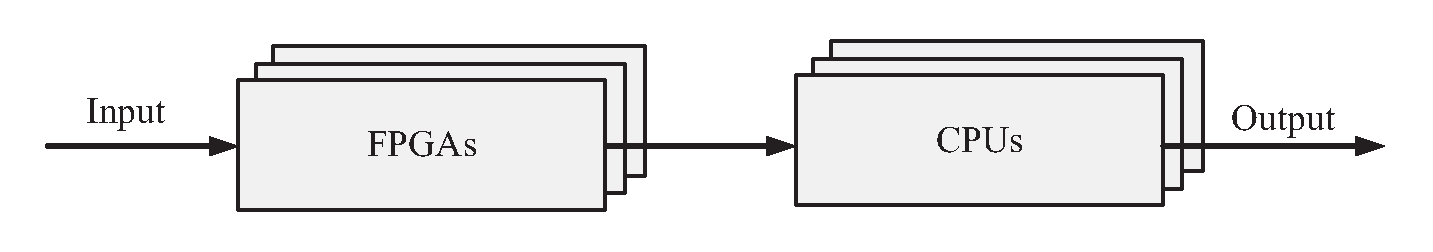
\includegraphics[width=0.7\textwidth]{1_introduction/figures/het_arch1}
	\label{fig:het_arch1}
}
\subfigure[]{
	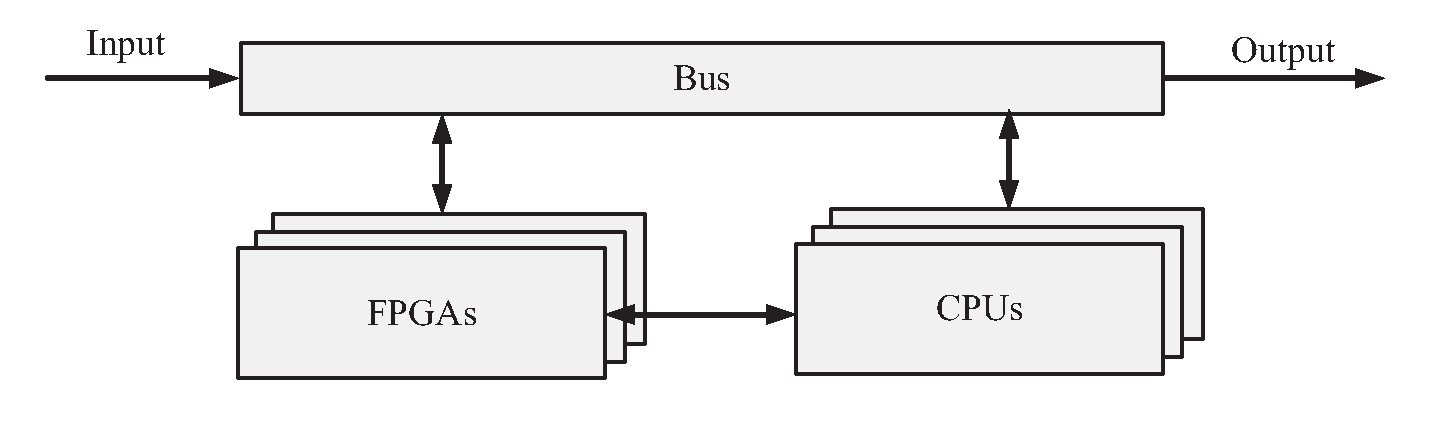
\includegraphics[width=0.7\textwidth]{1_introduction/figures/het_arch2}
	\label{fig:het_arch2}
}
\caption{Illustration of heterogeneous processing topologies: (a) Pre-processing by FPGAs; (b) Co-processing between FPGAs and CPUs.}
\label{fig:het_arch}
\end{figure}

The following three subsections present a brief overview of each contribution and the challenges involved.
More detail are presented in the later chapters.

\subsection{Precision Optimisation of Reconfigurable Data-paths}

The first contribution of this thesis is a \textit{precision optimisation approach to maximise real-time performance of reconfigurable systems}.

\glspl{fpga} have abundant fine-grained resources but the clock speeds of \glspl{fpga} are commonly 10 to 30 times slower than \glspl{cpu} and \gls{gpu},
therefore the performance gains in \glspl{fpga} are obtained by designing algorithms such that many independent operations can occur simultaneously.
A crucial step to unleash competitive performance of \glspl{fpga} is to provide massive parallelism and effective use of data.
By employing significant data-path parallelism and deep pipelines where inputs and outputs continually stream through each cycle, hundreds or even thousands of operations are executed on each cycle of \glspl{fpga} to outweigh the slow clock frequencies.
However, as each data-path requires replication of circuits and deep pipelines need numerous flip-flops, resource usage and bandwidth requirement are often the performance limitation for \gls{fpga} implementations~\cite{stitt11}.

Currently, \glspl{fpga} have the ability to support customisable data-paths with different precisions.
Reduced precision data-paths consume less logic resource and hence allow for a higher degree of parallelism.
Using reduced precision reduces I/O bandwidth and allows higher clock frequencies.
Unfortunately, all the mentioned benefits come with an expense of lower accuracy of results.
There are trade-offs between performance and accuracy in the implementation of data-paths.

Chapter~\ref{ch:precision} describes how reduced precision is applied to reconfigurable systems.
A novel data structure and memory architecture are developed.
They support reduced precision data-paths across multiple \glspl{fpga}.
They maintain the accuracy of final results by re-computing a small fraction of \gls{fpga} outputs on ~\glspl{cpu}.
This work employs the pre-processing topology (Figure~\ref{fig:het_arch1}), and the data-paths on \glspl{fpga} compute and filter most of the data before sending the filtered data to \glspl{cpu} for re-computation.

The proposed methodology is applied to an image-guided surgical robot application which employs the \gls{pq} process.
Functional transformation further optimises the data-path for hardware-friendly implementation.
Implementation in a reconfigurable platform with four \glspl{fpga} shows 58 times speedup over a 12-core \gls{cpu} system, 3 times speedup over a \gls{gpu} system, and 3 times speedup over the same reconfigurable platform without precision optimisation.

\subsection{Run-time Adaptation of System Configuration}

The second contribution of this thesis is \textit{an approach that adapts the reconfigurable systems at run-time for reduced computation workload and energy consumption}.

Power and energy efficiency is becoming a major consideration for ~\gls{hpc} systems.
%Since early 2000, the frequencies of \glspl{cpu} have hit a \textit{power wall}, which means that high power consumption prevents higher frequencies from being achieved on \glspl{cpu}.
For example, the Green500 list~\cite{green500} provides a ranking of the energy efficiency of world-wide supercomputers.
\glspl{cpu} are equipped with various technologies to reduce power dissipation~\cite{intelsleep,intelturboboost}.
\glspl{gpu} also have different power modes~\cite{amdpower,nvidiapower}.
As \glspl{fpga} are increasingly being deployed for \gls{hpc} applications, power dissipation of \glspl{fpga} is also a concern.
Apart from traditional power saving techniques such as clock gating and dynamic frequency/voltage scaling existing on other platforms, \glspl{fpga}' run-time reconfigurability could be exploited as an aggressive power saving technique.
The power consumption of an \gls{fpga} depends on the circuit size and the clock frequency.
Larger circuit uses more routing tracks which bring parasitic capacitance,
and higher clock speed increases the switching activity on the routing tracks which causes significant power dissipation.

Chapter~\ref{ch:adaptation} explores an adaptation approach to reduce \gls{fpga}'s energy consumption by run-time reconfiguration.
In particular, \gls{smc} applications are studied as they facilitate adaptation at algorithmic and system levels.
At algorithmic level, an adaptive \gls{smc} algorithm which adjusts the computation workload at run-time while maintaining the quality of results is proposed.
At system level, run-time reconfigurability of \glspl{fpga} is used to switch the real-time system between computation mode and low-power mode.
Low-power mode lowers the dynamic power by reducing circuit size and clock frequency.
Compared to a non-adaptive and non-reconfigurable system, the proposed approach reduces idle power by 25-34\% and the overall energy consumption by 17-33\%.

This work employs the co-processing topology (Figure~\ref{fig:het_arch2}), the \glspl{fpga} handle the computation which can be fully-pipelined, while the \glspl{cpu} deal with non-sequential data access.

\subsection{Design Flow for Domain-specific Reconfigurable Applications}

The final contribution of this thesis is \textit{the development of a design flow that reduces the development effort of real-time applications on reconfigurable systems}.

Although \glspl{fpga} show promising performance advantage for high-performance real-time systems, \gls{fpga} accelerators have not yet been accepted by mainstream application designers~\cite{stitt11}.
Low productivity and long design time have been a longstanding barriers to a more wide-spread usage.
The design complexity of \gls{fpga} applications far exceeds that of \glspl{cpu} and \glspl{gpu}, and hence raises development cost and deter user acceptance.
Traditionally, \gls{fpga} applications are developed using \glspl{hdl}.
Writing \glspl{hdl} is timing-consuming and requires digital design expertise which is not common to mainstream designers.
In addition, designers have to perform numerical analysis to determine an appropriate precision in order to achieve an \gls{fpga}'s full potential, because \glspl{fpga} often achieve order of magnitude improvements when using fixed-point, integer, or bit-level operations.
This numerical analysis process significantly increases design time.
Another productivity bottleneck is lengthy compilation times due to the complexity of placement and routing.
Common software design practices based on rapid compilation are no longer feasible for reconfigurable system design.

In Chapter~\ref{ch:tool}, a design flow is proposed to address the above mentioned challenge.
This chapter extends the \gls{smc} reconfigurable system described in Chapter~\ref{ch:adaptation} and focuses on making the system parametrisable for a wide variety of \gls{smc} applications.
In other words, it makes Chapter~\ref{ch:adaptation}'s reconfigurable system easier and more accessible to designers, especially those lack hardware design experience.
Through templating the \gls{smc} structure, the proposed design flow enables efficient mapping of applications to multiple \glspl{fpga}.
To reduce design space exploration effort, a machine learning algorithm based on surrogate modelling is used to tune design parameters that are crucial to the performance and solution quality.
The design flow demonstrates its capability of producing reconfigurable implementations for a range of \gls{smc} applications that have significant improvement in speed and in energy efficiency over optimised \gls{cpu} and \gls{gpu} implementations.


\section{Thesis Organisation}

\textbf{Chapter~\ref{ch:background}} offers a detailed background on reconfigurable architectures and systems, design flow which includes synthesis tools and programming languages, and applications of reconfigurable technologies on real-time systems.
\textbf{Chapter~\ref{ch:precision}} describes the first contribution, which demonstrates how precision optimisation is applied to reconfigurable real-time systems.
The proposed methodology is applied to an application in imaged-guided surgical robot based on \gls{pq} process. 
\textbf{Chapter~\ref{ch:adaptation}} presents the second contribution of this thesis, which describes the use of run-time reconfigurability of \glspl{fpga} to adapt real-time systems for reduced power and energy consumption.
\textbf{Chapter~\ref{ch:tool}} details the third contribution, which provides a design flow for automatically generating efficient implementation of reconfigurable designs.
Lastly, Chapter~\ref{ch:conclusion} concludes this thesis, and presents the remaining outstanding challenges.
Figure~\ref{fig:intro_organisation} shows how the three contributions of this thesis link together.
Chapter~\ref{ch:precision} and ~\ref{ch:adaptation} describe techniques to optimise reconfigurable real-time systems.
Chapter~\ref{ch:tool} introduces a domain-specific design flow to address the long-standing programmability issues of \gls{fpga}.

\begin{figure}[ht]
\begin{center}
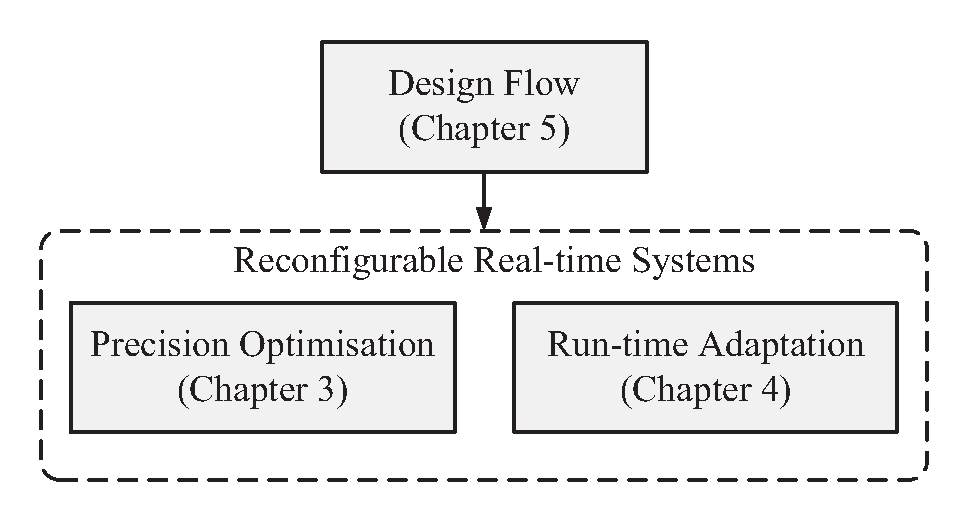
\includegraphics[width=0.7\textwidth]{1_introduction/figures/organisation}
\end{center}
\caption{Thesis organisation.}
\label{fig:intro_organisation}
\end{figure}

Parts of this thesis have been published in~\cite{chau13fpt,chau13arc,chau14trets,chau14fccm}.
During the course of this work, several related papers were also published.
Papers~\cite{chau13acm,eele13cdc,eele13gnc} describe details concerning the acceleration of air traffic management systems, one of the \gls{smc} applications being studied in Chapter~\ref{ch:tool}.
Paper~\cite{kurek14fccm} presents details of surrogate modelling that enable machine learning approach in Chapter~\ref{ch:tool}.
Papers~\cite{chau12fpl,niu13fccm} present initial work regarding the adaptive \gls{smc} method, which leads to the proposal in Chapter~\ref{ch:adaptation}.
Paper~\cite{chau12heart} provides a simple benchmarking platform for real-time systems.
Due to page limitations, neither of these contributions are described in this thesis.

\section{Statement of Originality}

I declare that this thesis was composed by myself, and that the work it presents is my own, except where otherwise stated.

